\documentclass{article}
\usepackage{amsmath}
\usepackage{graphicx}
\usepackage{float}
\usepackage{subcaption}
\usepackage{setspace}
\usepackage{siunitx}
\usepackage{multirow}
\usepackage{booktabs}
\usepackage{tikz}
\usepackage{pgfplots}
\usepackage{circuitikz}
\usepackage{fullpage}

\title{Lab 2 Report}
\author{Rayson Lim 1002026}
\date{\today}
\setcounter{tocdepth}{1}
\sisetup{
    round-mode = places,
    round-precision = 2
}
\usetikzlibrary{trees}
\pgfplotsset{width=\linewidth,height=0.6\linewidth,compat=1.14}

\begin{document}
    \maketitle
    \pagenumbering{arabic}

    \section{Results}
    	\subsection{Time taken for Mean calculations}
    	\begin{table}[H]
	    	\begin{center}
	    	\begin{tabular}{c | c }
	    	\textbf{Number of threads} & \textbf{Time(ms)} \\ \hline
	    	1 & 2.742 \\
			2 & 2.747 \\
			4 & 3.809 \\
			8 & 3.819 \\
			16 & 4.069 \\
			32 & 5.152 \\
			64 & 5.34 \\
			128 & 6.151 \\
			256 & 9.152 \\
			512 & 13.127 \\
			1024 & 22.221 \\
			2048 & 42.229 
	    	\end{tabular}
	    	\caption{Time taken to find Mean}
	    	\end{center}
    	\end{table}

    	\begin{figure}[H]
	    	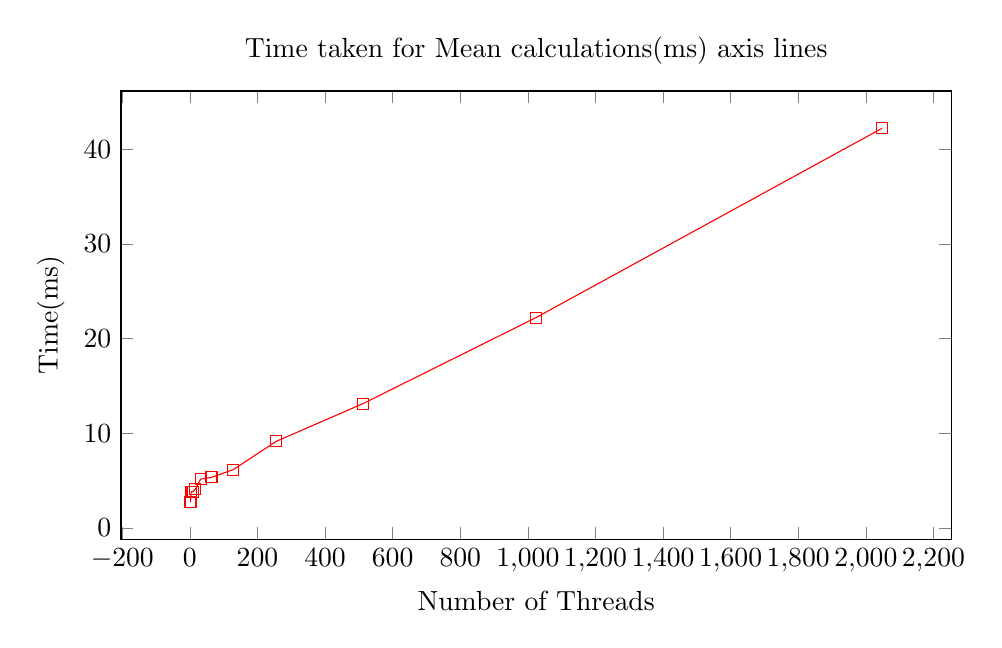
\begin{tikzpicture}
	  		\begin{axis}[
			    title = {Time taken for Mean calculations(ms)}
			    axis lines = left,
			    xlabel = {Number of Threads},
			    ylabel = {Time(ms)},
			    ]
			    \addplot [color=red, mark=square]coordinates {(1,2.742)(2,2.747)(4,3.809)(8,3.819)(16,4.069)(32,5.152)(64,5.34)(128,6.151)(256,9.152)(512,13.127)(1024,22.221)(2048,42.229)};
			\end{axis}  
			\end{tikzpicture}
			\caption{Scatter plot of results}
    	\end{figure}

    	\subsection{Time taken for Median calculations}
    	\begin{table}[H]
	    	\begin{center}
	    	\begin{tabular}{c | c }
	    	\textbf{Number of threads} & \textbf{Time(ms)} \\ \hline
	    	1 & 200.055 \\
			2 & 210.683 \\
			4 & 258.087 \\
			8 & 289.732 \\
			16 & 303.855 \\
			32 & 335.455 \\
			64 & 404.053 \\
			128 & 565.813 \\
			256 & 995.430 \\
			512 & 1529.267 \\
			1024 & 2847.666 \\
			2048 & 5511.868 
	    	\end{tabular}
	    	\caption{Time taken to find Median}
	    	\end{center}
    	\end{table}

    	\begin{figure}[H]
	    	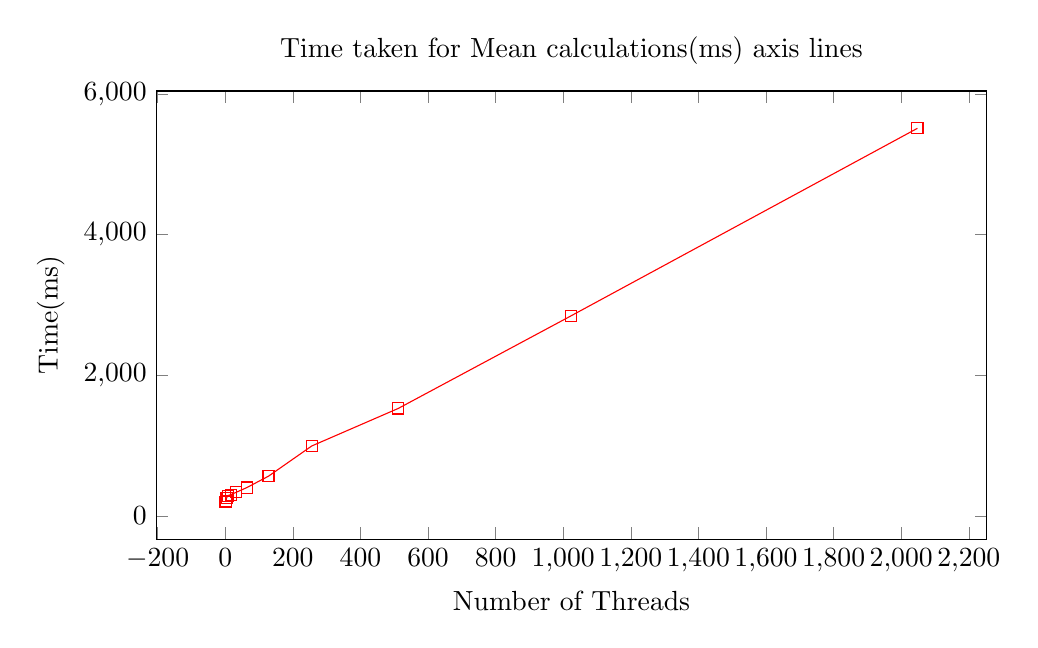
\begin{tikzpicture}
	  		\begin{axis}[
			    title = {Time taken for Mean calculations(ms)}
			    axis lines = left,
			    xlabel = {Number of Threads},
			    ylabel = {Time(ms)},
			    ]
			    \addplot [color=red, mark=square]coordinates {(1,200.005)(2,210.683)(4,258.087)(8,289.732)(16,303.855)(32,335.455)(64,404.053)(128,565.813)(256,995.430)(512,1529.267)(1024,2847.666)(2048,5511.868)};
			\end{axis}  
			\end{tikzpicture}
			\caption{Scatter plot of results}
    	\end{figure}

    \section{Screenshots}
    	\begin{figure}[H]
    		\centering
    		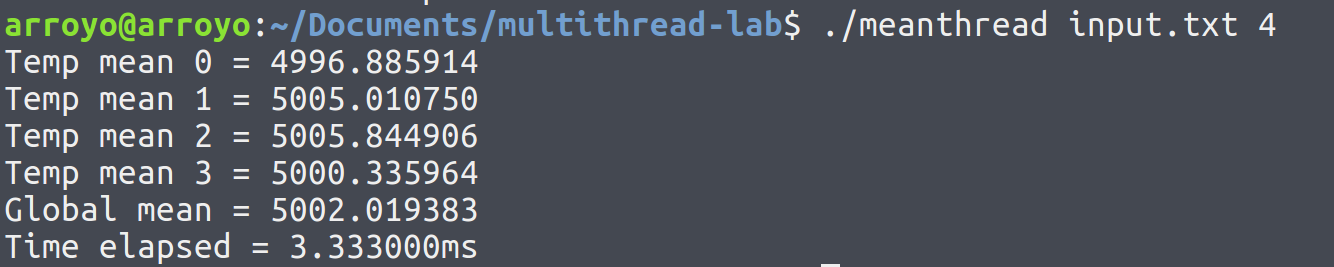
\includegraphics[width=\linewidth]{mean_screenshot.png}
    		\caption{Screenshot of mean calculator in action}
    	\end{figure}

    	\begin{figure}[H]
    		\centering
    		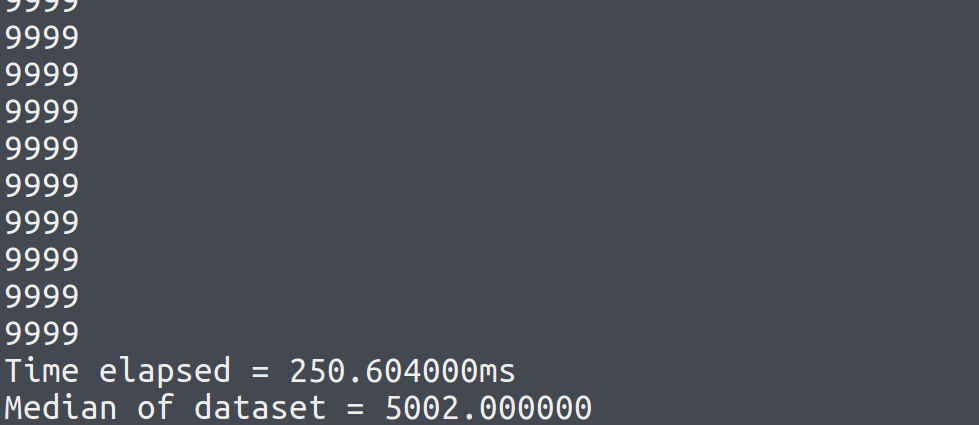
\includegraphics[width=\linewidth]{median_screenshot.png}
    		\caption{Screenshot of median calculator in action}
    	\end{figure}

\end{document}
